\section{Results}
\label{sec:results}

\begin{figure}[t]
\centering
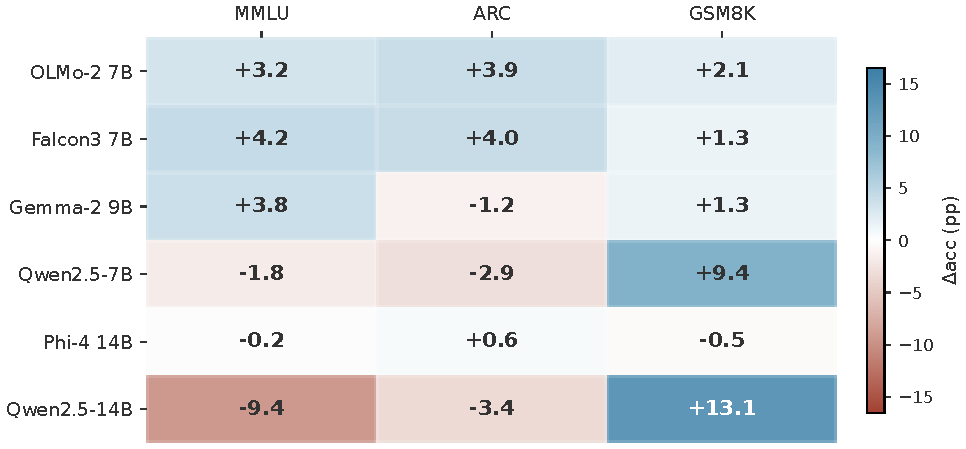
\includegraphics[width=0.88\columnwidth]{figures/fig_cross_benchmark_heatmap.pdf}
\caption{Cross-benchmark transfer at d100. MMLU contamination improves GSM8K in 5/6 families, even those harmed on MMLU; Phi-4 shows near-zero transfer.}
\label{fig:cross_benchmark_heatmap}
\end{figure}

Cross-family SFT-injection results (\S\ref{sec:taxonomy}) use seed$=$42 data across six models from five independent families ($\leq$3B dose-response in Appendix~\ref{sec:dose_response_details}). Within-family IRT analyses (\S\ref{sec:calibration_results}--\ref{sec:domain_differential}) use $J=16$ Qwen2.5 models (8$\times$1.5B + 8$\times$3B); domain-level contamination estimates $\gamma_d$ (\S\ref{sec:domain_differential}) are reported at $J=16$ in the text and $J=13$ in Figure~\ref{fig:domain_gamma}.

\subsection{Dose-Response Patterns}
\label{sec:taxonomy}

Applying Algorithm~\ref{alg:profile-classification} to seed$=$42 accuracy trajectories yields a spectrum of dose-response patterns (Table~\ref{tab:taxonomy}, Figure~\ref{fig:dose_response}), not a uniform inflation effect. Figure~\ref{fig:baseline_vulnerability} visualizes how contamination response correlates with baseline accuracy across families.

\paragraph{Replication status.}
Two patterns replicate across independent families (Table~\ref{tab:taxonomy}). \textit{Immune}: Phi-4 ($\pm$0.5pp), confirmed out-of-sample by LLaMA-3.1 ($-$0.69pp). \textit{Benefit}: three families gain $+$3.2 to $+$4.2pp (Gemma-2, Falcon3, OLMo-2 borderline; \S\ref{sec:cross_seed}). Two patterns are Qwen2.5-specific and await independent replication: Qwen-14B \textit{collapses} ($-$9.4 to $-$25.0pp across seeds) while Qwen-7B shows \textit{V-recovery}. ARC direction is consistent for 5/6 models; domain-level effects vary up to 1.8$\times$ (Appendices~\ref{sec:arc_cross_benchmark},~\ref{sec:domain_decomposition}).

\paragraph{Out-of-sample~validation.}
LLaMA-3.1-8B (Meta; d000, d025, d100) is classified Immune on both MMLU ($-$0.69pp) and ARC ($+$0.09pp), despite matching OLMo-2's Benefit baseline (53.5\% vs.\ 53.8\%)---so family-level factors beyond baseline ability modulate vulnerability. LLaMA-3.1 also shows the strongest GSM8K transfer ($+$16.4pp; Appendix~\ref{sec:gsm8k_dose_response}): target-benchmark immunity does not imply transfer immunity.

\subsection{Cross-Benchmark Transfer}
\label{sec:gsm8k_transfer}

\begin{table}[t]
\centering
\caption{Cross-benchmark transfer: MMLU vs.\ GSM8K accuracy change at d100. LLaMA-3.1 shows the strongest asymmetric transfer ($+$16.4pp GSM8K despite MMLU immunity). Gemma-2 excluded due to CoT collapse under MC-format SFT.}
\label{tab:gsm8k_transfer}
\footnotesize
\resizebox{\columnwidth}{!}{%
\begin{tabular}{lcccl}
\toprule
Model & MMLU $\Delta$ & GSM8K $\Delta$ & Range & Transfer \\
\midrule
Phi-4 14.7B & $\pm$0.5pp & $-$0.5pp$^{\diamond}$ & --- & Null \\
OLMo-2 7B & $+$3.2pp & $+$2.1pp$^{\S}$ & --- & Consistent \\
Falcon3 7B & $+$4.2pp & $+$1.3pp & --- & Consistent \\
Qwen-7B & $-$1.8pp & $+$9.4pp & $\pm$0.9 & Reversal \\
Qwen-14B & $-$9.4pp & $+$13.1pp & $\pm$7.4 & Reversal$^{\dagger}$ \\
LLaMA-3.1 8B & $-$0.7pp & $+$16.4pp$^{\ddagger}$ & --- & Asymmetric \\
\bottomrule
\multicolumn{5}{l}{\scriptsize $^{\dagger}$d000 baseline seed-sensitive (s42$=$60.8\% vs.\ s123$=$76.7\%); d100 stable ($82\pm0.5$\%).} \\
\multicolumn{5}{l}{\scriptsize $^{\S}$Mean of s42 and s123: $+$2.1pp (s42: $+$1.7pp, s123: $+$2.4pp); s0 excluded ($+$9.2pp outlier).} \\
\multicolumn{5}{l}{\scriptsize $^{\ddagger}$Single seed (s0); MMLU Immune but strongest GSM8K transfer across all families.} \\
\multicolumn{5}{l}{\scriptsize $^{\diamond}$Seed s123; Table~\ref{tab:gsm8k_dose} reports s0 ($+$1.14pp).}
\end{tabular}}
\end{table}

Contamination patterns are a property of the (model, benchmark) pair, not the model alone. Within-MC direction agreement is 86\% (6/7 models; Appendix~\ref{sec:arc_cross_benchmark}); across formats (MC$\to$generative math), agreement drops to 50\% with three families reversing on GSM8K \citep{cobbe2021gsm8k} (Table~\ref{tab:gsm8k_transfer}). Qwen-14B ($-$9.4pp MMLU) gains $+$13.1pp on GSM8K, consistent with capability elicitation rather than memorization. Volume effects are ruled out: d005 ($+$1.5\% data, seed$=$42) already yields $+$6.4pp GSM8K transfer for Qwen-7B.

\subsection{Cross-Seed Stability}
\label{sec:cross_seed}

\begin{figure}[t]
\centering
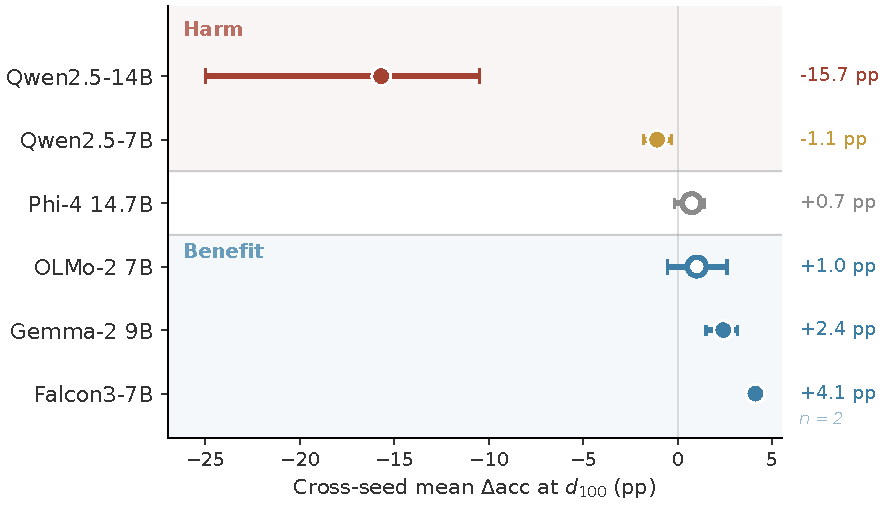
\includegraphics[width=\columnwidth]{figures/fig_cross_seed_ci.pdf}
\caption{Cross-seed mean $\Delta$acc at d100 with bias-corrected and accelerated (BCa) bootstrap 95\% CIs ($n\!=\!3$ seeds; Falcon3 $n\!=\!2$). Filled markers: CI excludes zero.}
\label{fig:cross_seed_ci}
\end{figure}

Gemma-2 is the only family with a statistically significant cross-seed Benefit (BCa 95\% CI $[+1.49, +3.14]$; Figure~\ref{fig:cross_seed_ci}); Falcon3 and OLMo-2 are directionally consistent but exploratory (Table~\ref{tab:cross_seed}). Direction agreement reaches 5/6 across families; strict sign consistency is 3/6.

\subsection{Item-Level Memorization Test}
\label{sec:memorization_test}

We test whether dose-response patterns arise from item-specific memorization using the treated/untreated split at d025 (3{,}540 / 10{,}502 MMLU items). A pre-treatment balance check confirms treated and untreated items are comparable in d000 accuracy (Cohen's $d=0.02$), difficulty distribution, and domain coverage (all $p>0.19$), supporting the parallel trends assumption. No model shows a significant difference-in-differences (DiD) effect ($p > 0.05$; Table~\ref{tab:did}), ruling out item-specific effects $>$2pp (MDES 1.25--2.05pp; ARC MDES in Appendix~\ref{sec:mdes}). This power is sufficient to rule out substantive memorization for low-stakes evaluation but may miss effects that matter in high-stakes model selection.

Parallel changes suggest global capability modulation (Figure~\ref{fig:treated_untreated}; multi-dosage analysis in Appendix~\ref{sec:did_dosage}).

\paragraph{Volume control.}
A volume-matched control (Falcon3-7B trained on 66{,}533 non-benchmark MC items; Appendix~\ref{sec:volume_control}) achieves 60.67\% MMLU, decomposing the $+$4.19pp Benefit into data quantity ($+$1.90pp, 45\%) and contamination content ($+$2.29pp, 55\%); ARC yields a consistent 43\%/57\% split; GSM8K shows 53\%/47\% ($+$0.68pp/$+$0.61pp of $+$1.29pp total). Collapse ($-$9.4pp) and Immune ($<$1pp) cannot arise from volume effects that produce $+$1.90pp in the control.

\begin{table}[t]
\centering
\caption{Cross-seed $\Delta$acc (d000$\to$d100). Strict sign consistency (Cons.) is 3/6; classification-level direction agreement is 5/6 (see text). Per-seed shape classification\textsuperscript{$\ddagger$} agrees for only 3/6.}
\label{tab:cross_seed}
\footnotesize
\resizebox{\columnwidth}{!}{%
\begin{tabular}{lcccccccl}
\toprule
Model & $n$ & s42 & s123 & s0 & 95\% CI & Dir. & Cons.\ & Pattern\textsuperscript{$\ddagger$} \\
\midrule
Phi-4 & 3 & 0 & $+$ & 0 & [$-$0.17, $+$1.39]\textsuperscript{B} & Immune & $\times$ & --- \\
Qwen-14B & 3 & $-$ & $-$ & $-$ & [$-$24.99, $-$10.49]\textsuperscript{B} & Harm & \checkmark & Collapse \\
Qwen-7B & 3 & $-$ & 0 & $-$ & [$-$1.82, $-$0.34]\textsuperscript{B} & Harm & $\times$ & V-recovery \\
Gemma-2 & 3 & $+$ & $+$ & $+$ & [$+$1.49, $+$3.14]\textsuperscript{B} & Benefit & \checkmark & Benefit \\
OLMo-2 & 3 & $+$ & 0 & $+$ & [$-$0.55, $+$2.60]\textsuperscript{B} & Borderl.\ & $\times$ & ---\textsuperscript{b} \\
Falcon3-7B & 2 & $+$ & $+$ & --- & [$+$3.91, $+$4.19]\textsuperscript{c} & Benefit & \checkmark & Benefit \\
\bottomrule
\multicolumn{9}{l}{\scriptsize \textsuperscript{B}BCa bootstrap ($B\!=\!10{,}000$); original five families at $n\!=\!3$.} \\
\multicolumn{9}{l}{\scriptsize \textsuperscript{$\ddagger$}Per-seed shape may differ from family-level direction-based classification (\S\ref{sec:classification}).} \\
\multicolumn{9}{l}{\scriptsize \textsuperscript{b}$+$/0/$+$ across seeds. Signs: $+$/$-$ = $|\Delta|{\ge}1$pp; $0$ = $|\Delta|{<}1$pp.} \\
\multicolumn{9}{l}{\scriptsize \textsuperscript{c}$n\!=\!2$ seeds only; range shown instead of BCa CI.}
\end{tabular}}
\end{table}

\subsection{Diagnostic Utility}
\label{sec:calibration_results}

Within-family IRT analysis uses Qwen2.5 $\leq$3B ($J=16$; ability separation in Appendix~\ref{sec:theta_separation}), where aggregate contamination shifts accuracy by ${\sim}$0.6--0.7pp. IRT is fitted on 300 randomly subsampled items (2.1\% of MMLU; representative by KS/$\chi^2$ tests, all $p > 0.5$); RRF exposure scoring achieves $\tau = 0.73$ ($\Delta\tau = 0.18$ vs.\ random; ablation in Appendix~\ref{sec:rrf_ablation}). A single-signal (Min-K\%++) pipeline shows severe model misfit (PPP $< 0.001$ vs.\ $0.193$; Appendix~\ref{sec:s2_only_pipeline}), confirming multi-signal fusion is essential.

ContamCal's primary diagnostic value lies in domain-level $\gamma_d$ estimates with credible intervals: Social Sciences $\gamma_d = -0.63$ ($P(\gamma_d\!<\!0) = 99.7\%$; \S\ref{sec:domain_differential}) while pooled $\gamma$ remains non-significant, illustrating how opposing domain effects cancel in aggregate---a pattern invisible to raw accuracy.

Table~\ref{tab:baselines} compares methods on 300 randomly subsampled items with RRF exposure scores. Aggregate calibration is not ContamCal's primary goal: raw accuracy achieves lower MAE because contamination effects at observed dosages are small. B6-DCR systematically overcorrects (MAE 0.108). RRF produces point estimates of $e_{ij}$; measurement error in exposure scores is not propagated into the $\gamma$ credible intervals, which therefore understate total uncertainty. Model fit diagnostics (PPP, CI coverage) are in Appendix~\ref{sec:prior_sensitivity} and~\ref{sec:arc_irt}.

\subsection{Detection Signal Failure Modes}
\label{sec:signal_failure}

Min-K\%++ \citep{zhang_2024_minkpp} exhibits \textit{directional reversal} at 0.5B: contaminated items receive \textit{lower} scores (paired Cohen's $d = -1.98$ at d100, $|d| > 1.2$ at d005). S1 achieves AUC $> 0.95$ at all scales; S4 is near-random below 1.5B (Appendix~\ref{sec:signal_reliability_appendix}). Simulation shows $\gamma$ recovery requires AUC$\geq$0.55 with $J \geq 50$; at AUC $\geq 0.90$, $J = 16$ suffices (Appendix~\ref{sec:identifiability_appendix}).

\subsection{Domain-Level Analysis}
\label{sec:domain_differential}

\begin{figure}[t]
\centering

\includegraphics[width=\columnwidth]{figures/fig_domain_gamma.pdf}
\caption{Per-domain $\gamma_d$ estimates with 95\% CIs ($J$=13 Qwen2.5; $J$=16 estimates differ by $<$10\%, Table~\ref{tab:domain_gamma}).}
\label{fig:domain_gamma}
\end{figure}

Within-family domain analysis (Qwen2.5, $J=16$) reveals directional heterogeneity masked by aggregate scores: STEM domains show positive $\gamma_d$ while Social Sciences is negative ($\gamma_d = -0.63$, 95\% Bayesian credible interval $[-1.07, -0.19]$, $P(\gamma_d\!<\!0) = 99.7\%$, PPP$=$0.722; Figure~\ref{fig:domain_gamma}, Table~\ref{tab:domain_gamma} in Appendix). Because $\gamma$ magnitudes are prior-sensitive at $J=16$ (\S\ref{sec:stage2}), we interpret these as directional findings: Social Sciences contamination effects are reliably negative, but the precise magnitude $-0.63$ should not be over-interpreted. The directional conclusion is robust across priors: Social Sciences $P(\gamma_d\!<\!0)$ is 99.35--99.85\% (Table~\ref{tab:socsci_prior}), exceeding the Bonferroni threshold ($99.375\%$) under baseline and loose priors but falling 0.025\,pp short under the tight prior $\mathcal{N}(0, 0.5)$. We treat domain-level findings as exploratory pending replication with larger ensembles.
